\documentclass[12pt,a4paper]{scrartcl}

% Bibtex setup {{{
\usepackage[utf8]{inputenc}
\usepackage{csquotes}
\usepackage[
  backend=biber,
  language=ngerman,
  style=chem-acs,
  bibstyle=chem-acs,
]{biblatex}
\addbibresource{sources.bib}
\DeclareFieldFormat{date}{\bfseries{#1}}
% }}}

% Packages, general {{{
\usepackage[ngerman]{babel}
\usepackage{siunitx}
\usepackage{setspace}
\usepackage{hyperref}
% }}}

% Packages, chemistry {{{
\usepackage{upgreek}
\usepackage{chemformula}
\usepackage{chemobabel}
\usepackage{chemfig}
\usepackage[formula={chemformula}]{chemmacros}
% }}}

% Document setup {{{
\onehalfspacing
\parindent0pt
\parskip6pt
% }}}

\begin{document} % {{{
\pagenumbering{gobble}
\begin{titlepage} % {{{
  \vspace*{6cm}
  \begin{center} % {{{
    \Large{\textbf{Anorganisch-Chemisches Praktikum}} \\
    \vspace*{1cm}
    \Large{Protokoll zur Darstellung von} \\
    \vspace*{1cm}
    \large{\textbf{Tetraamminkupfer(II)-sulfat Monohydrat} \ch{[Cu(NH3)4]SO4 * H2O}}
  \end{center} % }}}
  \vspace*{5cm}
  Name: Luca Zeuch \\
  Datum: \today \\
  Matrikelnummer: XXXXXX \\
\end{titlepage} % }}}

\pagenumbering{arabic}

\section{Einleitung} % {{{
Kupferkomplexe sind aufgrund ihrer strukturellen, magnetischen, Elektronentransfer- und katalytischen
Eigenschaften\textsuperscript{\cite{Singh:a12030}} von großem Interesse. Das in dieser Arbeit beschriebene Komplexsalz
wurde erstmalig 1644 von Johan Baptista van Helmont hergestellt\textsuperscript{\cite{meyer1905meyers}} und wird als
\textit{Kalkblau} oder \textit{Neuwieder Blau} für Malerfarben verwendet.\textsuperscript{\cite{brockhaus}}

In dieser Arbeit wird die Darstellung von Tetraamminkupfer(II)-sulfat Monohydrat beschrieben und die Eigenschaften der
Komplexverbindung herausgearbeitet.
% }}}

\section{Ergebnisse und Diskussion} % {{{
Es wurden 1.69\,g (6.00\,mmol) des Produkts erhalten, was einer Ausbeute von 60 \% entspricht. Verluste sind
möglicherweise durch das Waschen mit Ethanol zu erklären, da 96\%iger Ethanol verwendet wurde und somit ein Teil des
Produktes dort in Lösung gegangen sein könnte.

Ferner schlägt die Fachliteratur vor, das Produkt nicht nur zweimal mit Ethanol, sondern vorher mit einer
1:1-Mischung von Ethanol und konzentrierter Ammoniak-Lösung zu waschen.\textsuperscript{\cite{brauer1965handbook}}
Hierbei werden etwaige Verluste kleiner gehalten, da so das Lös\-lich\-keits\-pro\-dukt des Produktes schneller erreicht wird
und somit weniger in Lösung geht.

Gelöstes Kupfersulfat-Pentahydrat \ch{CuSO4 * 5 H2O} reagiert mit gelöstem Ammoniak \ch{NH3} zu
Tetra\-ammin\-kupfer(II)-sulfat Monohydrat unter Abspaltung des überschüssigen Kris\-tall\-wassers.\textsuperscript{\cite{brauer1965handbook}\cite{J/B:2022:tetkupf}}
\begin{reaction}
  CuSO4 * 5 H2O + 4 NH3 ->[ H2O ] \lbrack{}Cu(NH3)4\rbrack{}SO4 * H2O + 4 H2O
\end{reaction}

Die Treibkraft dieser Reaktion ist die Stabilität des Komplexes, da \ch{NH3} im Vergleich zum Aqua-Liganden ein
stärkerer Ligand ist.
% }}}

\section{Experimenteller Teil} % {{{
Es wurden 2.56\,g \ch{CuSO4 * 5 H2O} (10.0\,mmol, 1 Äquiv.) unter leichtem Erwärmen in circa 3\,mL destilliertem Wasser
gelöst. Anschließend wurde tropfenweise eine konzentrierte Ammoniak-Lösung hinzugegeben, bis sich der entstandene
tiefblaue Niederschlag wieder löste und man eine ebenso tiefblaue Lösung erhielt.

Diese Lösung wurde mit circa 3\,mL eines 1:1 Ethanol-Wasser-Gemisches überschichtet sowie mit weiteren 3\,mL 96\%igem
Ethanol. Das so präparierte Becherglas wurde abgedeckt und für sechs Tage an einem Ort mit möglichst wenig Luftbewegung
und Er\-schüt\-te\-rung\-en stehen gelassen.

Nach dieser Zeit hat sich ein blauer, kristalliner Niederschlag gebildet, der durch Filtration abgetrennt wurde.
Dieser Niederschlag wurde mehrfach mit 96\%igem Ethanol sowie abschließend einmal mit Diethylether gewaschen.
Nach dem Trocknen an Luft erhielt man ein feines, tiefblaues, kristallines Pulver.
% }}}

\section{Zusammenfassung} % {{{
Das Komplexsalz Tetraamminkupfer(II)-sulfat Monohydrat wurde erfolgreich synthetisiert und aufgereinigt. Die Synthese
hatte eine befriedigende\textsuperscript{\cite{vogel}} Ausbeute von 60\%. Das erhaltene Produkt hatte die zu erwartenden
Eigenschaften und konnte als tiefblaues, kristallines Pulver isoliert werden.
% }}}

\section{Zusatzfragen} % {{{
In Tetraamminkupfer(II)-sulfat Monohydrat hat \ch{Cu^{2+}} die Elektronenkonfiguration \ch{[Ar] 3d^9 4s^0}. Mit einem
ungepaarten Elektron ergibt sich für diesen paramagnetischen Komplex eine oktaedrisch-verzerrte Geometrie. Durch diese
Verzerrung wird das zweifach besetzte \ch{e_g}-Orbital energetisch abgesenkt, während das zweite \ch{e_g}-Orbital mit
einem Elektron energetisch angehoben wird. Dieser Effekt wird als Jahn-Teller-Effekt bezeichnet.

% TODO: Wie ist das Sulfat-Ion im Kristallgitter angeordnet?
\begin{figure}[htbp] % {{{
  \centering
  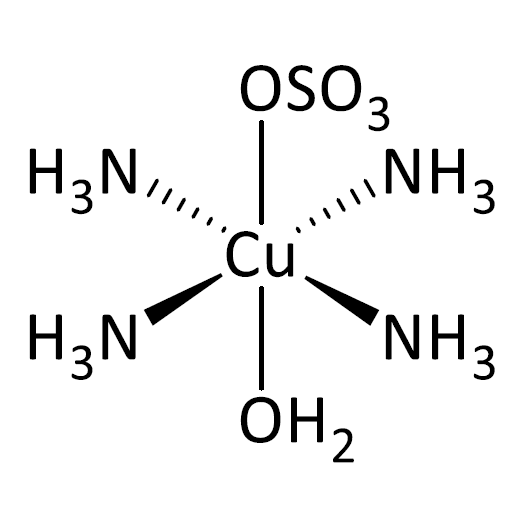
\includegraphics[width=0.5\textwidth]{images/crystal-cell.png}
  \caption{Kristallstruktur von Tetraamminkupfer(II)-sulfat Monohydrat.}
  \label{fig:struktur}
\end{figure} % }}}
% }}}

\newpage
\printbibliography
\end{document} % }}}

% vim:foldmethod=marker
